% !TeX root = ../main.tex

\chapter{编译器前端设计实现}

程序通常由程序员以文本形式输入,即字符序列。程序作为文本的表示称为具体语法。
我们用具体语法简明地写下和讨论程序的语法。
在编译器中,我们使用抽象语法树来表示程序,因为编译器可以很方便高效地操作抽象语法树。
翻译具体语法到抽象语法的过程称作解析。
本文不过多谈及解析的理论和实现,一方面是因为现阶段解析已经有了相对固定化的套路和工具,研究也已经趋于完善。
另一方面由于本文选择了 Racket 作为源语言和实现语言,我们可以很方便地从输入的本文序列中构造出结构体,
而 Racket 的结构体也是本文选择的用以表示抽象语法树的数据结构。

在本章中,我们通过一个简单的例子来说明如何表示语法,
如何使用Racket语言从文本中构造并操纵语法树,
然后给出本文实现的语言的完整语法。

\section{抽象语法树和文法}

在计算机科学中,抽象语法树,或简称语法树,是源代码语法结构的一种抽象表示。
它以树状的形式表现编程语言的语法结构,树上的每个节点都表示源代码中的一种结构。
之所以说语法是“抽象”的,是因为这里的语法并不会表示出真实语法中出现的每个细节。
比如,嵌套括号被隐含在树的结构中,并没有以节点的形式呈现;
而类似于 if-condition-then 这样的条件跳转语句,可以使用带有三个分支的节点来表示。

编程语言可以被看作是合法程序的集合,这一集合通常是无限大的,因为我们总是可以写出更加庞大复杂的程序。
因此,我们无法简单地通过把所有的合法程序列出来来描述一门语言。
通常,我们使用文法——一系列规则,来构造程序。文法通常用来描述具体语法,但它也可以被用来描述抽象语法。
本文使用巴科斯-诺尔范式\cite{Knuth_1964, Backus_Bauer_1960}的变体来描述我们的语言。
图\ref{fig:con-syntax-eg}中的几条规则给出了本文实现的语言的一个子集的描述,
该语言仅支持包含加减法的整数运算,但它允许任意复杂的嵌套表达式。
其中 \code{read} 函数读取用户在键盘上输入的一串数字,返回一个整数。

\begin{figure}[t]
  \fbox{
    \begin{minipage}{0.96\textwidth}
      \[
      \begin{array}{rcl}
        \Type & ::= & \key{Integer} \\
        \Exp & ::= & \Int \MID \LP\key{read}\RP \MID \LP\key{-}\;\Exp\RP \MID \LP\key{+} \; \Exp\;\Exp\RP \\
        \Lang & ::= & \Exp
      \end{array}
      \]
    \end{minipage}
  }
  \caption{具体语法示例}
  \label{fig:con-syntax-eg}
\end{figure}

\begin{figure}[t]
  \fbox{
    \begin{minipage}{0.96\textwidth}
      \[
      \begin{array}{rcl}
        \Type & ::= & \key{Integer} \\
        \Exp &::=& \INT{\Int} \MID \READ{} \MID \NEG{\Exp} \\
        &\MID&  \ADD{\Exp}{\Exp}  \\
        \LangInt{}  &::=& \PROGRAM{\code{'()}}{\Exp}
      \end{array}
      \]
    \end{minipage}
  }
  \caption{抽象语法示例}
  \label{fig:abs-syntax-eg}
\end{figure}


下面这行代码是这个示例语言的一个合法的程序:

\begin{lstlisting}
(+ (read) (- 8))
\end{lstlisting}

该程序对应的语法树如图\ref{fig:ast-eg}。

\begin{figure}[t]
  \begin{center}
      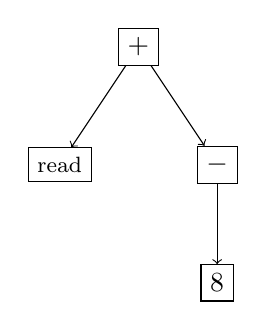
\begin{tikzpicture}
        \node[draw] (plus)  at (0 ,  0) {\key{+}};
        \node[draw] (read)  at (-1, -1.5) {{\footnotesize\key{read}}};

        \node[draw] (minus) at (1 , -1.5) {$\key{-}$};
        \node[draw] (8)     at (1 , -3) {\key{8}};

        \draw[->] (plus) to (read);
        \draw[->] (plus) to (minus);
        \draw[->] (minus) to (8);
      \end{tikzpicture}
  \end{center}
  \caption{语法树示例}
  \label{fig:ast-eg}
\end{figure}

\section{构造和操纵语法树}

我们使用Racket的结构体来表示语法树,
用抽象语法来描述各个结构体的定义,
用Racket的模式匹配来构造和操纵语法树。

图\ref{fig:con-syntax-eg}对应的抽象语法的描述如图\ref{fig:abs-syntax-eg}所示。
其中\code{Int},\code{Prim}等即为对应的Racket结构体的构造函数。
这些结构体可以非常简单地被定义出来:
\begin{lstlisting}
(struct Int (value))
(struct Prim (op args))
\end{lstlisting}

构造结构体也非常简单,下面这行代码对应的即为具体语法为\code{(+ (read) (- 8))}的程序:
\begin{lstlisting}
(Prim '+
      (list (Prim 'read '())
            (Prim '- (list (Int 8))))
\end{lstlisting}

而对结构体使用模式匹配,我们可以很方便地判断结构体的类型以及访问结构体的成员,也就是语法树的子树。
例如,对于下面这段代码
\begin{lstlisting}
(match ast
  [(Prim op (list child1 child2))
   (print op)])
\end{lstlisting}
将对变量\code{ast}进行模式匹配,如果变量是一个包含两个(可能复杂的)操作数的语法树,就打印操作符。
同时,这段代码还会将两个操作数,也就是两个子树,分别绑定到变量\code{child1}和\code{child2}上去。
例如,如果\code{ast}的值是\code{(+ (read) (- 8))},
则\code{child1}和\code{child2}的值将分别被赋值为\code{(read)}和\code{(- 8)},
并且代码将打印出\code{+}。

一个模式匹配当然也可能包含多个子句,这些子句将会从上到下依次被判断是否匹配。
例如,下面这个\code{leaf?}函数接受一个名为ast的参数,判断该它是否是叶子节点:
如果是一个数字或者\code{read}函数,则为叶子节点;如果是加运算或者取负运算,则不是叶子节点。
\begin{lstlisting}
(define (leaf? ast)
  (match ast
    [(Int n) true]
    [(Prim 'read '()) true]
    [(Prim '- (list e1)) false]
    [(Prim '+ (list e1 e2)) false]))
\end{lstlisting}

以下三行代码的返回值将分别为 \code{true, false, true}:
\begin{lstlisting}
(leaf (Prim 'read '()))
(leaf (Prim '- (list (Int 8))))
(leaf (Int 8))
\end{lstlisting}

接下来我们看一下如何使用模式匹配,配合Racket的\code{read}函数来构造语法树。
事实上,Racket提供的各种reader本身就已经是一个递归下降解析器。
\code{read}函数接收一个输入端口,返回一个包含数值和符号的list。
例如,假设一个源代码文件中存放了上面的例子中的代码:\code{(+ (read) (- 8))}。
对这个文件调用\code{read}函数会返回这样的一个list:
\code{('+ ('read) ('- 8))}。单引号表示这是一个符号。
模式匹配可以对list和符号进行匹配。

\begin{lstlisting}
(define (parse e)
  (match e
    [(? symbol?) (Var e)]
    [(? fixnum?) (Int e)]
    [`(,op ,es ...)
     (Prim op (map parse es))]
    ...
    ))
\end{lstlisting}

上面的\code{parse}函数就可以从list中构造出我们想要的语法树。
如果它接收的参数是符号,则返回一个变量节点;
如果是整数,则返回一个整数节点;
如果是一个运算,则对操作数列表递归调用\code{parse}函数,
将返回的节点作为运算结构体的成员,也就是作为该节点的各个子树。
如此我们就利用Racket的reader和模式匹配实现了编译器的前端部分。

\section{源语言语法}

在语言特性的选择上,我们主要考虑让它们能尽可能地体现不同的编译原理的知识面。
对于基本数据类型,本文实现了 64 位整数及其加、减、乘、整除、模运算,布尔类型及其与、或运算;
本文没有实现浮点数与浮点运算,因为它们只是单纯地覆盖了更多的 x86-64 指令,
并不会增加语言的表现力;
本文没有采用纯函数式的方式,而是支持了可变变量和循环,
因为这会迫使我们在进行数据流分析时考虑循环数据流;
对于复合数据结构,本文仅实现了向量(元组),
向量是一个存放在堆上的、定长的、允许存放不同类型元素的结构,
这足以让我们考虑堆上的内存数据和垃圾回收;
最后是函数,本文实现了一等函数,利用向量实现了闭包,并且在翻译过程中正确地处理了尾递归。

在类型系统方面,本文没有实现类型推导,但只有函数的形式参数以及返回值需要显式声明类型,
其余变量(即局部变量)定义时并不需要声明类型。
例如,如下的代码是一个合法的程序。
该程序从键盘读取一个(大于0的)整数,如果是偶数则返回1,奇数则返回0。
\begin{lstlisting}
(define (even? [x : Integer]) : Boolean
  (if (eq? x 0)
      #t
      (odd? (- x 1))))

(define (odd? [x : Integer]) : Boolean
  (if (eq? x 0)
      #f
      (even? (- x 1))))

(if (even? (read)) 1 0)
\end{lstlisting}


图\ref{fig:full-concrete-syntax}展示了源语言完整的具体语法。



\newcommand{\GrammarRacket}{
  \begin{array}{rcl}
    \Type &::=& \key{Integer} \MID
                \key{Boolean} \MID
                \key{Void} \MID
                \LP\key{Vector}\;\Type \ldots \RP \\
          &\MID& (\Type \ldots \; \key{->}\; \Type) \\

    \itm{bool} &::=& \TRUE \MID \FALSE \\
    \itm{op} &::=& \key{+} \MID \key{-} \MID \key{*} \MID \key{quotient} \MID \key{remainder} \MID \key{and} \MID \key{or} \MID \key{not} \\
    \itm{cmp} &::= & \key{eq?} \MID \key{<} \MID \key{<=} \MID \key{>} \MID \key{>=} \\

    \Exp &::=& \Int{} \MID \itm{bool} \MID \Var \MID \CREAD \MID \LP\key{void}\RP \\
          &\MID& \CNEG{\Exp} \MID (\itm{op}\;\Exp\;\Exp) \MID (\itm{cmp}\;\Exp\;\Exp) \\
          &\MID& \CLET{\Var}{\Exp}{\Exp} \MID \CIF{\Exp}{\Exp}{\Exp} \\
          &\MID& \CSETBANG{\Var}{\Exp} \MID \CBEGIN{\Exp}{\ldots} \MID \CWHILE{\Exp}{\Exp} \\
          &\MID& \LP\key{vector}\;\Exp \ldots \RP \MID \LP\key{vector-length}\;\Exp\RP \\
          &\MID& \LP\key{vector-ref}\;\Exp\;\Int\RP \MID \LP\key{vector-set!}\;\Exp\;\Int\;\Exp\RP \\
          &\MID& \LP \key{procedure-arity}~\Exp\RP \\
          &\MID& \CLAMBDA{\LP\LS\Var \key{:} \Type\RS\ldots\RP}{\Type}{\Exp} \\
    \Def &::=& \CDEF{\Var}{\LS\Var \key{:} \Type\RS \ldots}{\Type}{\Exp} \\

    \Lang{} &::=& \Def\ldots \; \Exp\ldots
  \end{array}
}


\begin{figure}[t]
  \fbox{
    \begin{minipage}{0.96\textwidth}
      \[
\begin{array}{lcl}
  \GrammarRacket{}
\end{array}
      \]
    \end{minipage}
  }
  \caption{源语言的完整语法}
  \label{fig:full-concrete-syntax}
\end{figure}
